\renewcommand{\labelitemi}{$\bullet$}
\renewcommand{\labelitemii}{$\cdot$}
\renewcommand{\labelitemiii}{$\diamond$}
\renewcommand{\labelitemiv}{$\ast$}

\section{Introduction à la théorie du contrôle métabolique}

\paragraph{Outline}
\begin{itemize}
	\item Introduction à l'analyse de la sensibilité systémique
	\item Un exemple simple
	\item La matrice stœchiométrique
	\item L'évolution du système
	\item Les coefficients de contrôle
	\item \textit{Summation theorem}
	\item Coefficients de réponse et d'élasticité
	\item Théorème de connectivité
\end{itemize}


\paragraph{Problème général}
\begin{itemize}
	\item Prenons un \textcolor{blue}{réseau métabolique complexe arbitraire}
	\item Chaque vitesse de réaction répond au changements de concentrations en substrats, produits et quelque effecteurs :
	\begin{itemize}
		\item Ces lois cinétiques ont des \textcolor{blue}{propriétés moléculaires particulières}
	\end{itemize}
	\item Questions importantes du MCT :
	\begin{itemize}
		\item Comment le système réponds aux changements des propriétés moléculaire individuelle (activités des enzymes) ?
		\item Comment la réponse du système dépend de la \textcolor{blue}{structure du réseau} ?
		\item Comment sont contraintes les sensibilités systémiques ? Est-ce qu'elles montrent des dépendances ?
	\end{itemize}
\end{itemize}
\textit{Quelles répercutions au systèmes entier par rapport aux propriétés individuelles ?}


\paragraph{État stationnaire et définition du système}
Le métabolisme est une usine chimique, une fonction durable pour traiter les nutriments et produire de la biomasse, énergie, déchets, etc. Il doit atteindre un \textbf{état stationnaire stable} (contrainte).

Donc :
\begin{itemize}
	\item Le système \textbf{doit être ouvert} afin d'atteindre un état stationnaire non-trivial réalisable thermodynamiquement (i.e, avec des flux non-nuls).
	\item La plupart des réactions doivent être sensible à la concentration des substrats et des produits, permettant la balance de la production de métabolites et des taux de consommations (équilibre entre flux entrants et sortant).   	
\end{itemize}


\paragraph{Raisonnement intuitif ?}
\begin{figure}
	\centering
	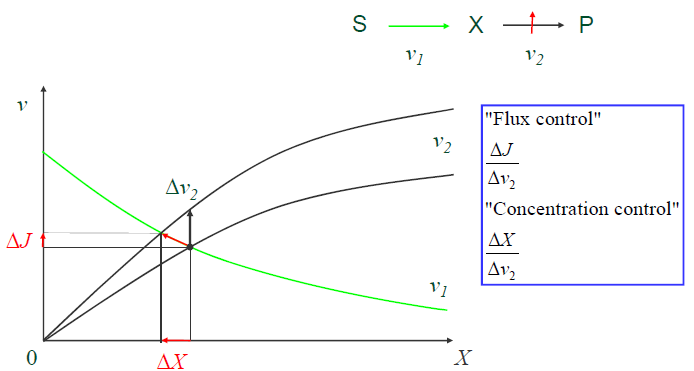
\includegraphics{Images/02_1.PNG}
\end{figure}
$X$ est un métabolite intermédiaire. L'état stationnaire est atteint  lorsque $v_1 = v_2$ = intersection des deux courbes. 
Le changement de flux dans ce cas est plus petit que le changement de vitesse de la seconde réaction. 


\paragraph{Quantitativement ?}
\begin{figure}
	\centering
	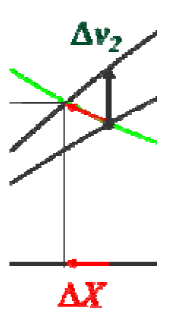
\includegraphics{Images/02_2.PNG}
\end{figure}
Prenons $E_2$ l'activité de l'enzyme 2. A l'état stationnaire :
$$ v_1(X,E_1) = v_2(X,E_2) $$
$$ \frac{\partial v_1}{\partial x} \Delta X \simeq \frac{\partial v_2}{\partial x} \Delta X + \frac{\partial v_2}{\partial E_2} \Delta E_2 $$

à la limite :
\textbf{Contrôle de la concentration} : \fbox{$\frac{\partial X}{\partial E_2} = \frac{-1}{\frac{\partial v_2}{\partial x}- \frac{\partial v_1}{\partial x}} $}
si $v_2$ et $E_2$ sont exprimés dans les mêmes unités. 


\paragraph{Quantitativement ?}
\begin{figure}
	\centering
	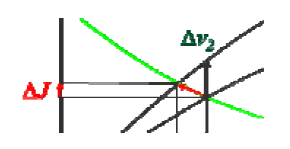
\includegraphics{Images/02_3.PNG}
\end{figure}
$$ J=v_2(X,E_2) $$
$$ \Delta \simeq \frac{\partial v_2}{\partial x} \Delta X + \frac{\partial v_2}{\partial E_2} \Delta E_2 $$

à la limite :
\textbf{Contrôle du flux} : \fbox{$\frac{\partial J}{\partial E_2} = \frac{\frac{\partial v_1}{\partial x}}{\frac{\partial v_2}{\partial x}- \frac{\partial v_1}{\partial x}} $}


\paragraph{Quantitativement ?}
Si nous modulons $E_1$ on obtient de manière similaire :

\fbox{	$  \frac{\partial X}{\partial E_1} = \frac{1}{\frac{\partial v_2}{\partial x}- \frac{\partial v_1}{\partial x}} $
$\frac{\partial J}{\partial E_1} = \frac{\frac{\partial v_2}{\partial x}}{\frac{\partial v_2}{\partial x}- \frac{\partial v_1}{\partial x}} $ }

Le contrôle du flux par l'apport de la réaction 1 est proportionnel à la sensibilité .........
\textit{Flux control by supply reaction 1 is proportional to sensitivity of demand reaction 2 to intermediate metabolite}


\paragraph{Quantitativement ?}
et nous obtenons la \textbf{relation de sommation} suivante : 
\fbox{ $ \frac{\partial X}{\partial E_1} + \frac{\partial X}{\partial E_2} = 0 $}
\fbox{$ \frac{\partial J}{\partial E_1} + \frac{\partial J}{\partial E_2} = 1 $ }

Contrôle de la concentration selon l'offre et la demande : signes opposés
Concentration control by supply and demand of opposite signs

Contrôle du flux selon l'offre et la deande ...
Flux control by supply and demand add up to 1


\paragraph{Plus généralement}
Il est possible d'obtenir un traitement général de la théorie du contrôle du système métabolique de \textbf{complexité arbitraire}. \textit{C. Reder (1988) J. Theoret. Biol. 135:175-201} 

\textbf{Définitions générales}:
\begin{tabular}{ll}
	$x = x(t,p)$ 	&	vecteur de concentrations, fonction du temps et des paramètres \\
	$X = X(p)$ 	&	vecteur de concentrations à l'\textbf{état stationnaire} : $dx/dt=0$ \\
	$v=v(x,p)$	&	vecteur des vitesse, fonction des molarités et des paramètres (\textit{expression inétique du système}) \\
	$J=J(p) = v(X(p),p)$	&	vecteur de flux à \textbf{l'état stationnaire}
\end{tabular}


\paragraph{La matrice stœchiométrique $N$}
\begin{itemize}
	\item Les réactions du réseau sont exprimés dans la matrice stœchiométrique $N$, où les colonne continnent les coefficients stœchiométriques de chaque réaction.
	\item Cette matrice reflète la \textbf{structure du système}
	\item N est de rang maximal si et seulement s'il n'y a pas de relation de conservation contraignant les différentes concentrations, que nous allons supposer initialement pour simplifier
	\item Sinon, elle peut être réduite à une matrice $N^0$ avec un rang maximal afin de traiter avec des variables indépendantes : $$ N=L.N^0 $$
\end{itemize}


\paragraph{Évolution du système}
L'évolution du vecteur de concentration $x$ du système est une fonction simple du vecteur de vitesse $v$ :

\fbox{ $ \frac{dx}{dt}=N.v(x,p)$} où $p$ est un vecteur de paramètres, incluant l'activité des enzymes.

La Jacobienne est :	$$ \textswab{J}  = N. \frac{ \partial v}{\partial x}     $$

$\frac{\partial v_i}{\partial x_j} $ : 'élasticités' non-normalisées


\paragraph{Contraintes des flux à l'état stationnaire}
Nous sommes intéressé par l'analyse de l'état stationnaire du système :
		$$ dx/dt = N . v(X(p),p) = 0 $$
où $X(p)$ est le vecteur des concentrations à l'état stationnaire.

L'état stationnaire introduit des \textbf{dépendances linéaires} entre les flux : 
$$ N. J(p) = 0 $$
Loi de Kirchhoff pour les métabolites intermédiaires 

Donc le vecteur de flux $J$ peut être exprimés dans la base de $Ker(N)$ (souvent appelé $K$) 


\paragraph{Contrôle de l'expression systémique}

Faisons la différence entre l'équation de l'état d'équilibre par rapport à $p$ :
$$ N . \frac{\partial v}{\partial x} . \frac{ \partial X}{\partial p} + N . \frac{\partial v}{\partial p} = 0 $$
\fbox{$ \frac{\partial X}{\partial p} = - (N. \frac{\partial v}{\partial x})^{-1} . N . \frac{\partial v}{\partial p} $}

\fbox{$ \frac{\partial X}{\partial p} = - \textswab{J}^{-1} . N . \frac{\partial v}{\partial p} $}

Cette équation relie les \textbf{changements systémiques} dans l'état stationnaire des concentrations $X$ aux changements de vitesse $v$.

La matrice $ \Gamma = - (N. \frac{\partial v}{\partial x})^{-1} . N  = - \textswab{J}^{-1} . N $ contient tous les \textbf{coefficient de contrôle des concentrations}.


\paragraph{Contrôle des flux}
Let us calculate the resulting steady-state flux : (MAL DIT) 
	$$ J=c(X(p),p) $$
and differentiate it respect to $p$ :
\begin{align*}
	\partial J / \partial p & = \partial v / \partial x . \partial X / \partial p + \partial v / \partial p \\
							& = ( \partial v / \partial x . \Gamma + I ) . \partial v/ \partial p 
\end{align*}

Cette équation relie les changements systémiques dans l'état stationnaire des flux $J$ aux changements de vitesses $v$.

La matrice $ \Phi = I + \partial v / \partial x . \Gamma $ contient tous les \textbf{coefficients de contrôle du flux}. 



\paragraph{Généralisation}
Si le système montre des \textbf{relations de conservation} comme $[ATP]+[ADP]+[AMP] = constante$, nous devons réduire la matrice $N$ à la matrice $N^0$ avec un rang maximal correspondant à une molarité des métabolites indépendants $x^0$.
\begin{align*}
	N & = L. N^0 \\
	dx^0/dt &= N^0 . v(x,p) \\
	\textswab{J} &= N^0 . \partial v / \partial x . L \\
	\Gamma & = - L . \textswab{J} ^{-1} . N^0 \\
	\Phi = I + \partial v / \partial x . \Gamma
\end{align*}




\paragraph{Coefficients de contrôle normalisé}

Il est de coutume d'exprimer le contrôle en termes de coefficients de contrôle \textbf{normalisés} sans dimension :

\begin{tabular}{rr}
	Contrôle du flux	&	$C_i^j = \frac{E_i}{J_j} \frac{\partial J_j}{\partial E_i } = \frac{\partial ln J_j}{\partial ln E_i}$ \\
	Contrôle des concentrations	&	$C_i^{X_j} = \frac{E_i}{X_j} \frac{\partial X_j}{\partial E_i } = \frac{\partial ln X_j}{\partial ln E_i}	$ \\
\end{tabular}

où les paramètres $E_i$ dénote les \textbf{activités enzymatiques}, en général exprimé dans les mêmes unités que $J_i (M.s^{-1})$.
